\def\year{2019}\relax
%File: formatting-instruction.tex
\documentclass[letterpaper]{article} %DO NOT CHANGE THIS
\usepackage{aaai18}  %Required
\usepackage{times}  %Required
\usepackage{helvet}  %Required
\usepackage{courier}  %Required
\usepackage{url}  %Required
\usepackage{graphicx}  %Required
\usepackage{hyperref}
\usepackage{amsmath}
\usepackage{amsfonts}
\usepackage{natbib}
\usepackage{xcolor}
\frenchspacing  %Required
\setlength{\pdfpagewidth}{8.5in}  %Required
\setlength{\pdfpageheight}{11in}  %Required
%PDF Info Is Required:
\setcounter{secnumdepth}{0}  

\usepackage[ruled,vlined]{algorithm2e}
\newcommand{\TODO}[1]{{\color{red}TODO: {#1}}}

\def\state{s}
\def\statet{\state_t}
\def\statetp{\state_{t-1}}
\def\statehist{\state_{1:t-1}}
\def\statetn{\state_{t+1}}
\def\obs{\meas}
\def\obst{\obs_t}
\def\act{a}
\def\actt{\act_t}
\def\acttp{\act_{t-1}}
\def\acttn{\act_{t+1}}
\def\Obs{\mathcal{O}}
\def\ObsEnc{\Phi_o}
\def\ObsProb{P_o}
\def\ObsFunc{C}
\def\ObsFuncFull{\ObsFunc(\statet, \actt) \rightarrow \obst}
\def\ObsFuncInv{\ObsFunc^{-1}}
\def\ObsFuncInvFull{\ObsFuncInv(\obst, \statetp, \actt) \rightarrow \statet}
\def\State{\mathcal{S}}
\def\Action{\mathcal{A}}
\def\TransP{P_{T}}
\def\Trans{T}
\def\TransFull{\Trans(\statet, \actt) \rightarrow \statetn}
\def\TransObs{T_c}
\def\Rew{R}
\def\rew{r}
\newcommand{\vect}[1]{\mathbf{#1}}
\def\rewards{\vect{r}_{1:t}}
\def\rewt{\rew_t}
\def\rewtp{\rew_{t-1}}
\def\rewtn{\rew_{t+1}}
\def\RewFull{\Rew(\statet, \actt) \rightarrow \rewtn}
\def\TransObsFull{\TransObs(\statet, \obst, \actt, \rewt; \theta_T) \rightarrow \statetn}
\def\Value{V}
\def\pit{\pi_t}
\def\piDef{\pi(\acttn|\statet, \obst, \actt, \rewt; \theta_\pi) \rightarrow \pit(\acttn ; \theta_\pi)}
\def\Valuet{\Value_t}
\def\ValueDef{\Value(\statet, \obst, \actt, \rewt; \theta_\Value) \rightarrow \Valuet(\theta_\Value)}
\def\R{\mathbb{R}}
\def\E{\mathbb{E}}
\newcommand{\meas}{z}
\newcommand{\measurements}{\vect{\meas}_{1:t}}
\newcommand{\meast}[1][t]{\meas_{#1}}
\newcommand{\param}{\theta}
\newcommand{\policy}{\chi}
\newcommand{\graph}{G}
\newcommand{\vtces}{V}
\newcommand{\edges}{E}
\newcommand{\st}{\state}
\newcommand{\stn}{\st_{t+1}}
\newcommand{\stt}{\st_t}
\newcommand{\stk}{\st_k}
\newcommand{\stj}{\st_j}
\newcommand{\sti}{\st_i}
\newcommand{\St}{\mathcal{S}}
\newcommand{\Act}{\mathcal{A}}
\newcommand{\acti}{\act_i}
\newcommand{\lpt}{\delta}
\newcommand{\trans}{P_T}
\newcommand{\Q}{\qValue}
\newcommand{\V}{V}
\newcommand{\fw}{\fwcost}

\newcommand{\fwcost}{F}
\newcommand{\qValue}{Q}
\newcommand{\prew}{\Upsilon}
\newcommand{\epiT}{T}
\newcommand{\vma}{\alpha_\Value}
\newcommand{\qma}{\alpha_\qValue}
\newcommand{\prewma}{\alpha_\prew}
\newcommand{\fwma}{\alpha_\fwcost}
\newcommand{\maxValueBeam}{\vect{\state}_{\Value:\text{max}(m)}}
\newcommand{\nil}{\emptyset}
\newcommand{\discount}{\gamma}
\newcommand{\minedgecost}{\fwcost_0}
\newcommand{\goal}{g}
% The file aaai.sty is the style file for AAAI Press 
% proceedings, working notes, and technical reports.
%
\title{Floyd-Warshall Reinforcement Learning: \\Combining advantages from
model-free and model-based RL}
\author{Vikas Dhiman}
\pdfinfo{
/Title ()
/Author ()}
\begin{document}

\maketitle
\begin{abstract}
Reinforcement Learning (RL) algorithms are often discriminated on the
basis of whether a state-transition model is learned implicitly
(\emph{model-free}) or explicitly (\emph{model-based}). In the implicit
case i.e.\ \emph{model-free} RL, algorithms such as Q-learning and
policy gradients learn a joint state-action function that maps
state-action pairs to expected future reward in an agent's environment.
The reward distribution that governs an agent's environment is thus
implicity memorized in the learning of this function.  Due to this
combined learning of state-transition dynamics and the reward
distribution, learned behaviors in \emph{model-free} RL are hard to
transfer to environments where the state-transition model remains the
same while the reward-distribution changes.  In contrast,
\emph{model-based} RL explicity learns the state transition function
allowing for the decoupling of learned behaviours to environments in
which only the reward distribution changes. Oftentimes, this explicit
modelling leads to the requirement of an additional planning step to
compute model dynamics which can make policy computation in such
algorithms expensive.  Inspired by both these RL paradigms and the
Floyd-Warshall algorithm for path-planning on graphs, we propose
Floyd-Warshall Reinforcement Learning (FWRL), a novel algorithm that
combines advantages from both \emph{model-based} and \emph{model-free}
approaches. Our main contribution is an algorithm that learns a
goal-conditioned value function which transitions from model-based
behavior to model-free behavior in well explored regions of an agent's
state space.  We show that FWRL transfers knowledge about the
environment when the reward location is dynamic compared to a
model-based Q-learning baseline.  We show (\TODO{fill in the results
when exp done}) that FWRL meets the ground between model-free and
model-based algorithms by being model-free in the more frequently
visited regions while being model-based on less visited paths.

%The Reinforcement learning algorithms are classified on the basis of whether
%the state-transition model is learned explicitly into \emph{model-based}
%and \emph{model-free} algorithms.
%%
%The \emph{model-free} algorithms like Q-learning and policy gradients are easier to learn in cases when model is more complex than the policy.
%However, model-free algorithms are harder to transfer in cases when the reward function changes while the state-transition model remains the same.
%The \emph{model-based} algorithms learn the state-transition model explicitly hence making it
%easier to separate the environment transition from the reward distribution.
%However, model-based algorithms require an additional planning step on the model dynamics
%which make it expensive to compute the policy.
%%
%We propose a novel algorithm that is based on a combination of model-free and model-based approaches.
%Due to it's similarity to Floyd-Warshall algorithm in path-planning on graphs, we call
%it Floyd-Warshall reinforcement learning (FWRL).
%We show that FWRL transfers the knowledge about the environment when the reward location is dynamic as compared to the model-based Q-learning algorithm.
%We show (\TODO{fill in the results when exp done}) that FWRL meets the ground between model-free and model-based algorithms by being model-free in the more frequently visited regions while being model-based in less visited paths.
\end{abstract}


\section{ Introduction}

The Reinforcement learning algorithms are classified on the basis of whether
the state-transition model is learned explicitly into \emph{model-based}
and \emph{model-free} algorithms.
%
The \emph{model-free} algorithms like Q-learning and policy gradients are easier to learn in cases when model is more complex than the policy.
However, model-free algorithms are harder to transfer in cases when the reward function changes while the state-transition model remains the same.
One example of such a problem is traveling salesman problem.
Although classical traveling salesman problem is a posed as a planning problem where the space has already been explored, however it is not hard to recognize that someone has to create a map of the map through exploration and sometimes it has to be the agent them-self.
In such a scenario, the traveling salesman has a dynamic reward with a static map that needs to be
explored.
The model-free approach fails to generalize to new rewards in these scenarios, because of the conflated representation of environment model and resulting reward.
In spite of these limitations, model-free approaches have been applied to multi-goal navigation
scenarios with considerable success \cite{mirowski2018learning}.
However, all these methods depend upon exploring the entire space being a candidate goal space.
Not only model-free approaches are sample inefficient, multi-goal navigation problem exaggerates this problem.

The \emph{model-based} algorithms learn the state-transition model explicitly hence making it
easier to separate the environment transition from the reward distribution. Also model-based
algorithms are known to be sample efficient than model-free algorithms especially in cases when
the state-transition model is translation invariant in the environment. 
However, model-based algorithms require an additional planning step on the model dynamics
which make it expensive to compute the policy on the fly.
Although model-based algorithms fail to find an optimal policy, because small errors in models can add up and lead to wrong prediction over larger state spaces. 

Taking inspiration from the Floyd-Warshall algorithm in graph-based path planning domain,
we propose Floyd-Warshall reinforcement learning (FWRL) algorithm that combines the
benefits of both model-based and model-free methods.
We define the Floyd-Warshall function $\fwcost$ for a goal state $\state_j$ starting from a
state-action pair $\state_i$, $\act_i$
as the expected reward through all possible paths $p_{ij}$ between the starting and
destination state while following policy $\pi_{j}$ to the destination $j$.
%
\begin{multline}
\fwcost(\state_j | \state_i, \act_k) \\
= \E_{p_{ij} \sim \pi_{j}}\left[
\sum_{\state, \act \in p_{ij} } \discount^{t} r(\state, \act) \right| p_{ij} = (\state_i, \act_k, \dots, \state_J) \Biggr] \, .
\end{multline}
%

Due to this formulation, the optimal Floyd-Warshall function should satisfy the transitive property
\begin{align}
\fwcost^*(\state_i, \act_i, \state_j) = \max_{\state_k} \left[
\fwcost^*(\state_i, \act_i, \state_k)
+ \max_{\act_k}\fwcost^*(\state_k, \act_k, \state_j) \right]
\label{eq:transitive-fw}
\end{align}

The advantage of this formulation is that as soon as the goal state $\state_g$, the Q-function and
hence the policy can be estimated from $Q(\state, \act) = F(\state, \act, \state_g) + \Rew(\state_g)$.
Even if the path between two states has not been ever traversed, the value function
can be computed using the transitive property in Eq~\ref{eq:transitive-fw}. 

In our experiments, we show how our approach is better than both model-free Q-learning and model-based approaches. We also show how our approach can be switch between either approaches depending upon traversal experience in the state space.

\subsection{Claims}
\begin{itemize} \item
Using FWRL is better than model-free learning like Q-learning in terms of generalizing to dynamic goals, static maps.
\item 
Using FWRL is better than model-based learning because of less accumulation over long term, hence more accurate value functions.
\item FWRL is better than Hindsight Experience Replay (HER) \cite{andrychowicz2016learning} because it is a parametric representation of hindsight.
\item FWRL is better than TDM~\cite{pong2018temporal} because it does not require the distance reward function.
\end{itemize}

\section{Related work}
\subsection{Goal-conditioned value functions}
The idea of goal-conditioned value function is not new but has got attention because of revival of reinforcement learning based on deep neural networks.
We build upon the goal-conditioned value functions of \citet{schaul2015universal}.
\citet{schaul2015universal} proposed an architecture and a matrix factorization based algorithm for faster learning of UVFA (Universal value function approximators).
UVFA focused on fast estimation of goal-conditioned value functions using sparse
matrix factorization but not on bridging the gap between model-based and model-free
algorithms.


\citet{andrychowicz2016learning} introduced the idea of Hindsight experience replay (HER) two learn about the model from previous episodes even when the goal location has changed or not been achieved.
Our method can be seen as parametric approximation of ``Hindsight memory'',
that can help compress information from previous episodes instead of maintaining the
entire history of replay memory.

\cite{pong2018temporal} propose temporal difference models that estimate goal directed Q function for a specific kind of reward function, in particular the distance from the goal and in contrast with limited temporal horizon.

\subsection{Combining model-based and model-free methods}



\subsection{Navigation with mapping}
 (1) CMP from Saurabh Gupta: is metric, might not working in continuous spaces.
 (2) Semi-parameteric Topological mapping: is not end to end.
 (3) Neural Map: Is actually not mapping

\subsection{Model free DRL }
does not generalize to multi-goal environments.

\subsection{Model based DRL}
Needs more exploration.
Find the paper that shows that Model based DRL can actually compete with Model free DRL as long as it models uncertainty.

\subsection{Multi-goal navigation based papers}
Mirowski 2017, 2018: No one shot map learning, does not generalizes to new maps.

\section{Problem definition}
\newcommand{\Rgoal}{R_{\text{goal}}}
Let the agent and its environment be represented by a state space $\State$ and the
agent can traverse through state space by taking actions $\act \in \Act$ in a
fixed action space $\Act$. At every time step $t$, the agent takes action $\act_t$
and observes state $\state_t \in \State$ and reward
$\rew_t \in [-\Rgoal, \Rgoal]$.
Consider an episode of $T$ time steps.
For every episode the environment chooses one of the states in the state space is
the goal state $\goal \in \State$.
We want to find the sequence of actions to take that
maximizes the total reward over $T$ time steps.
Once the agent reaches the goal $\|\state_t - \goal\| < \delta$, the agent receives the highest reward possible $\Rgoal$ in the game and gets respawned in the environment at a randomg \emph{spawn} state.
This cycle continues enabling the agent to reach the goal multiple times,
incentivizing rapid exploration and finding the shortest path to the goal.
For the new episode a new goal location is chosen, but rest of the environment stays the same.
The agent is allowed to remember about the environment from previous episode and use
it for this episode.

%
\begin{align}
\policy^*(\state_t ; \goal) = \act^*_t = \arg \max_{\act_t} \E_{\policy}\left[ \sum_{t=0}^T \rew_t \right]
\end{align}%
%

\subsection{Why is this problem important?}
Many real world problems can be formulated in this context.
Consider a traveling postman problem who has moved into a new city. The postman has
to explore the city and find the buildings that match the given address.
The next time the postman gets the same address, they can use their experience to find out the building.
Even when a new address is provided (in the next episode), the postman can use
experience to find the new episode more quickly.

In robotics, tasks like picking and placing the object at a desired location can be
formulated as goal-directed navigation.

\subsection{Why is the problem hard?}
Model-free Reinforcement learning methods assume that the rewards are being sampled
from the a static reward function.
In a problem where the goal location changes, hence the reward function also changes,
it becomes hard to transfer the learned value-function or action-value function to
the changed location.
One alternative is to concatenate the goal location the state, making the new state space
$[\state_t, \goal]^\top \in \State^2$ larger.
This method is wasteful in computation and more importantly in sample complexity.

\section{Method}
We present a model-free reinforcement learning method that easily transfers when goal
location is dynamic.
We accomplish this by maintaining a path based expected reward function from any state to any goal state.
We call this algorithm Floyd-Warshall Reinforcement Learning, because of its
similarity to Floyd-Warshall algorithm : a shortest-path planning algorithm on graphs.
We define Floyd-Warshall value function as
%
\begin{align}
\fwcost_{\policy}(i, l,  j) =
\E_{\policy}\left[ \sum_{t=0}^{t=k} \rew_t \middle\vert \state_0 = i, \act_0 = l, \state_k = j \right] .
\end{align}%
%
When the policy is optimal, the Floyd-Warshall function should satisfy the constraint
%
\begin{align}
\fwcost^*(\state_i, \act_i, \state_j) = \max_{\state_k} \left[
\fwcost^*(\state_i, \act_i, \state_k)
+ \max_{\act_k}\fwcost^*(\state_k, \act_k, \state_j) \right] .
\end{align}%
%

We summarize the algorithm in Alg~\ref{alg:floyd-warshall-small}.

\section{Experiments}
We setup two environments in the grid world and windy grid world.
\subsection{Four room grid world}

Four room grid world is a grid world with four rooms connected to each other as shown in Figure~\ref{fig:four-room-grid-world}.

\subsection{Four room windy world}

Four room windy world is a grid world with four rooms connected to each other as shown in Figure~\ref{fig:four-room-grid-world}.
Some of the grid cells in have wind shown by arrow and the agent gets pushed around by
the wind with 0.25 probability irrespective of the action taken.


%
\begin{figure}%
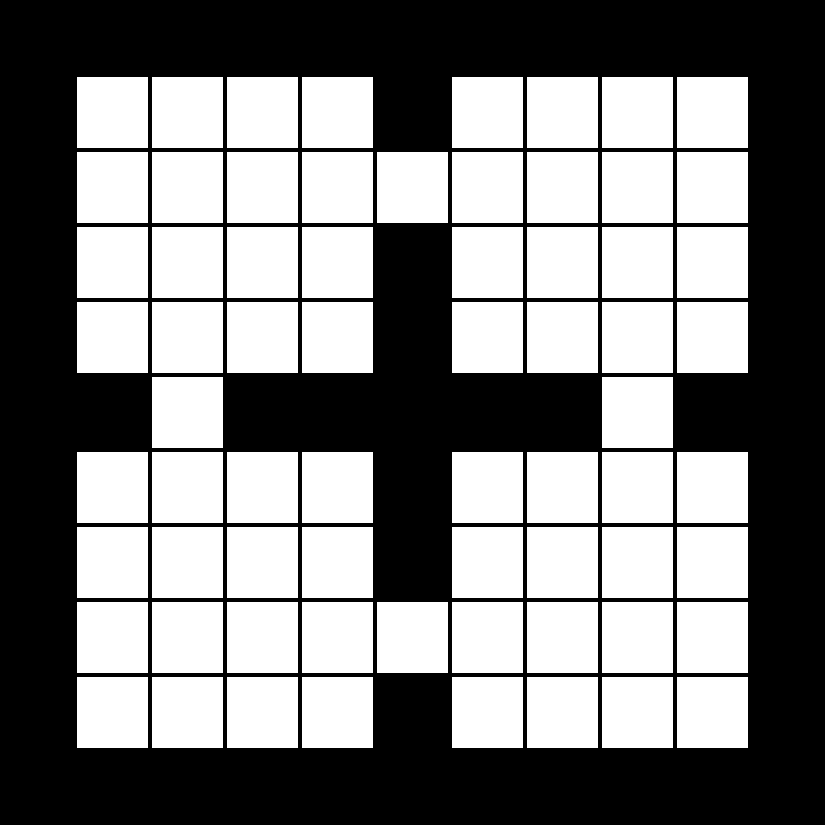
\includegraphics[width=0.48\columnwidth]{media/4-room-grid-world.pdf}
\hfill
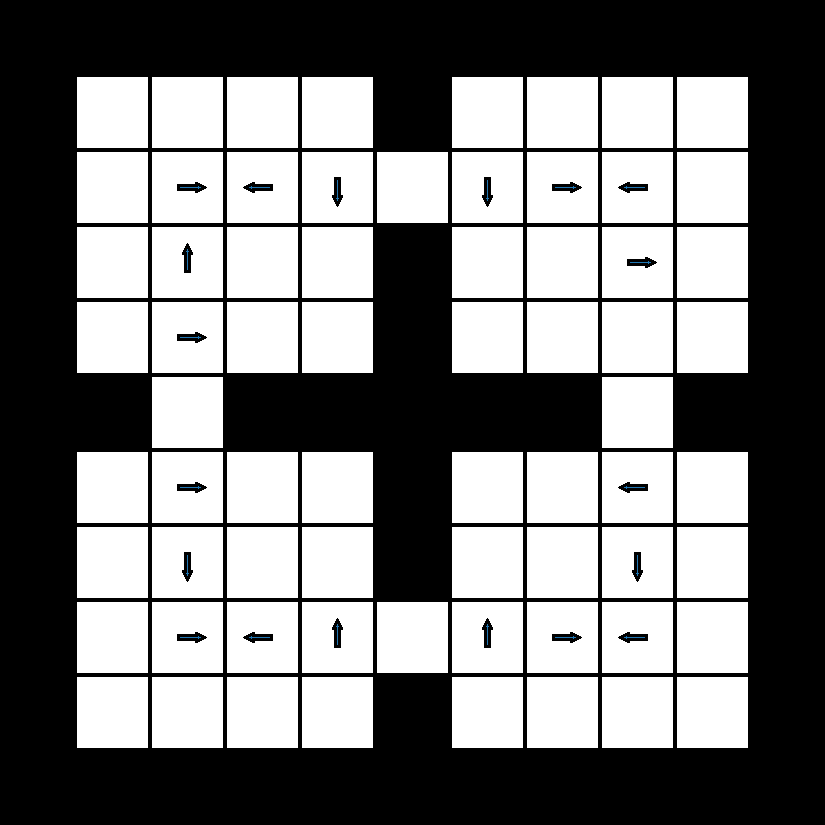
\includegraphics[width=0.48\columnwidth]{media/4-room-windy-world.pdf}%
\caption{Left: Four room grid world. Right: Four room windy grid world with wind direction shown by arrows. The windy pushes the agent in the direction of wind with 0.25 probability irrespective of the action taken.}
\label{fig:four-room-grid-world}%
\end{figure}%
%

\section{Results}

Fig~\ref{fig:ql-fw-grid-world-results} and Fig~\ref{fig:ql-fw-windy-world-results} show the results.

\begin{figure}%
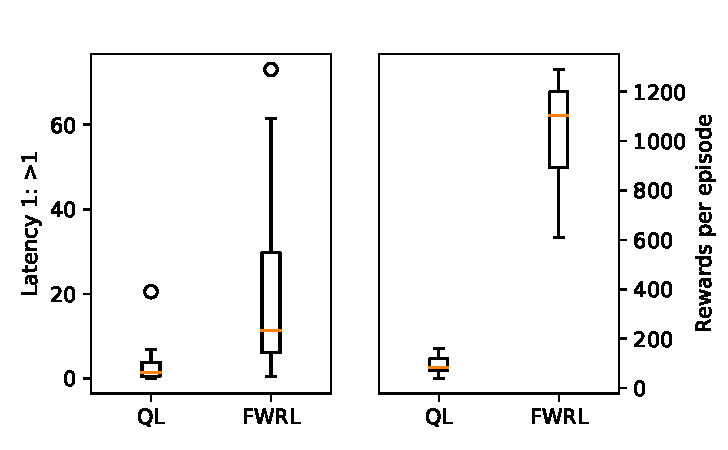
\includegraphics[width=\columnwidth]{./media/ql-fw-grid-world.pdf}\\
\caption{Results on Grid world}
\label{fig:ql-fw-grid-world-results}%
\end{figure}
\begin{figure}
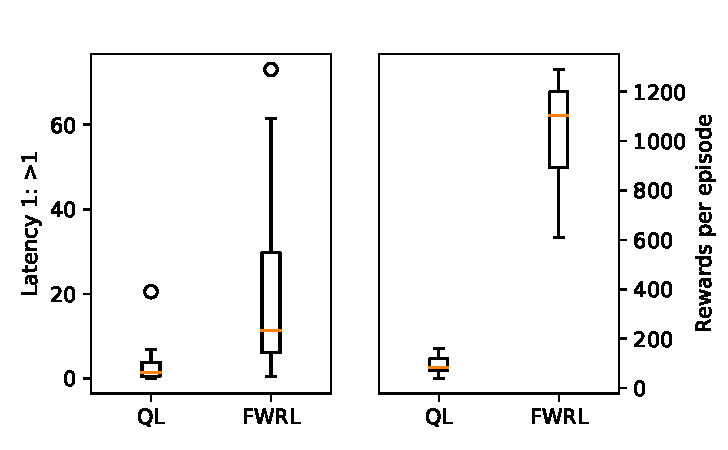
\includegraphics[width=\columnwidth]{./media/ql-fw-windy-world.pdf}%
\caption{Results on windy world}
\label{fig:ql-fw-windy-world-results}%
\end{figure}


\subsection{Future work}
Items to improve the algorithm:
\begin{itemize} \item
\TODO{Justify the computational cost of constraint} The cost of going through the entire state space.
How do you extend to a network? and large state spaces.
\begin{enumerate}\item
Observation 1: If there is only one goal, then the computation should not be any more than Q-learning.
This can be accomplished by assuming that transitivity is satisfied till
$\state_{t-1}$ and needs to be extend to only the next step. This sounds similar to the
 Floyd-Warshall dynamic programming update.
However, this assumes that $\state_t$ is being visited for the first time.
If the state $\state_t$ is being visited for the second time, the earlier
value may be the shorter path for it.
\end{enumerate}
\item
We need Q-value for exploration.
\end{itemize}

\begin{function}
\eIf{$\state_g = \phi$ or $\text{all}(\fwcost(\state_t, :, \state_g) = -\infty)$ }{
  \tcc{Exploration mode}
  $\act^* = \arg\max_{\act} Q(\state_t, \act)$\;
}{
  \tcc{Exploitation mode}
  $\act^* = \arg\max_{\act} F(\state_t, \act, \state_g)$\;
}

\caption{$\policy^*$($\state_t$, $\state_g$, $Q(., .)$, $\fwcost(.,.,.)$)}
\label{func:policy}
\KwRet{$\act^*$}
\end{function}

\begin{algorithm}
  Let $\rew_g \leftarrow 10$\;
  \tcc{By default all states are unreachable}
  Initialize $\fwcost(\state_i, \act_i, \state_j; \param_{\fwcost}) \leftarrow -\infty$ \;
  Initialize $Q(\state_i, \act_i) \leftarrow 1$ \;
  Initialize $\state_g = \phi$ \;
  Set $t \leftarrow 0$\;
  Observe $\meas_t$ \;
  $\state_t = \ObsEnc(\meas_t; \param_E)$ \;
  \For{$t \leftarrow 1$ \KwTo $\epiT$}{
  \tcc{See Function~\ref{func:policy}}
    Take action $\act_{t-1} \sim \text{Egreedy}(\policy^*(\state_{t-1}, \state_g, Q, \fwcost))$ \;
    Observe $\meas_t$, $\rew_t$ \;
    $\state_t = \ObsEnc(\meas_t; \param_E)$ \;
    \If{$\rew_t >= \rew_g$}{
      \tcc{Reached the goal}
      $\state_g \leftarrow \state_t$ \;
      \tcc{Respawning does not need update of value functions}
      continue\;
    }
    $Q(\state_{t-1}, \act_{t-1}) \leftarrow \rew_t + \max_{\act} Q(\state_t, \act)$ \;
    $\fwcost(\state_{t-1}, \act_{t-1}, \state_t) \leftarrow \rew_t$ \;
    \For{$\state_k \in \State, \act_k \in \Act, \state_l \in \State$}{
      $\fwcost(\state_k, \act_k, \state_l) \leftarrow
        \max \{
        \fwcost(\state_k, \act_k, \state_l),
        \fwcost(\state_k, \act_k, \state_t)
        + \max_{\act_p \in \Act} \fwcost(\state_t, \act_p, \state_l)
        \}$
        \;
    }
  }
  \KwResult{$\policy^*(\state_k, \state_g, Q, \fwcost)$}
  \caption{\small Floyd-Warshall Reinforcement Learning (Tabular setting)}
  \label{alg:floyd-warshall-small}
\end{algorithm}

\begin{itemize}\item
Grid world: Set up a random goal static maze scenario, compare with normal Q-learning.
\item
Lava world: Set up a Lava world like \cite{schaul2015universal} and test on it.
\item
\TODO{Atari games}: Compare performance with normal Q-learning.
\item
\TODO{Deepmind Lab}: Set up a random goal static maze scenario, compare with normal Q-learning. 
\end{itemize}



\def\localbib{/home/dhiman/wrk/group-bib/shared}
\IfFileExists{\localbib.bib}{
\bibliography{\localbib,main_filtered,main}}{
\bibliography{main_filtered,main}}
\bibliographystyle{aaai}
\end{document}
